\documentclass{llncs}
\usepackage{amsmath}
\usepackage{amssymb}
\usepackage{tikz}
\usetikzlibrary{arrows,automata}

\begin{document}

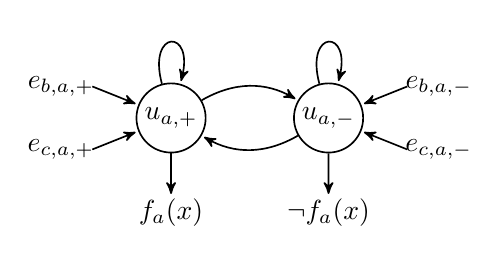
\begin{tikzpicture}[->,>=stealth',shorten
>=1pt,auto,node distance=2cm, semithick, initial text=,inner sep=0pt, minimum
size=0pt] 
		\node[state] (A+) {$u_{a, +}$};
		\node[state] (A-) [right of=A+] {$u_{a, -}$};

		\path (A+) edge[bend left] (A-)
		      (A+) edge[loop above] (A+);
		\path (A-) edge[bend left] (A+)
		      (A-) edge[loop above] (A-);

		\draw (A+) -- (0, -1); 
		\draw (A-) -- (2, -1); 
		\node at (0, -1.2) {$f_a(x)$};
		\node at (2, -1.2) {$\neg f_a(x)$};

		\draw (-1, 0.4) -- (A+);
		\draw (-1, -0.4) -- (A+);
		\draw (3, 0.4) -- (A-);
		\draw (3, -0.4) -- (A-);
		\node at (-1.4, 0.4) {$e_{b, a, +}$};
		\node at (-1.4, -0.4) {$e_{c, a, +}$};
		\node at (3.4, 0.4) {$e_{b, a, -}$};
		\node at (3.4, -0.4) {$e_{c, a, -}$};

		\end{tikzpicture}

\end{document}